\subsection{\secState{D}Emergency Head-On}\label{s:testEmergencyHeadOn}

\paragraph{Scenario:} Two  \emph{UAS} systems are flying in  \emph{uncontrolled airspace} (altitude $\le$ 500 ft. Above the Ground Level) with missions defined in (tab. \ref{tab:missionSetupEmergencyHeadOnScenario}). Both \emph{UAS} are in the  \emph{Navigation mode} with active \emph{ADSB-In/Out}, receiving position notifications from each other. Cruising altitude is sufficient for horizontal separation (50-100 ft. Above Ground Level). \emph{Horizontal separation} is preferred mode for both \emph{UAS}.


\begin{table}[H]
    \centering
    \begin{tabular}{c||c|c||c}
        \multirow{2}{*}{UAS} &\multicolumn{2}{c||}{Position} & \multirow{2}{*}{$\mathscr{WP}_1$} \\\cline{2-3}
          & $[x,y,z]$           & $[\theta,\varpi,\psi]$           & \\\hline\hline
        1 & $[0,20,0]^T $       & $[0^\circ,0^\circ,0^\circ]^T$    & $[40,20,0]^T$\\\hline 
        2 & $[40,20,0]^T $       & $[0^\circ,0^\circ,180^\circ]^T$  & $[0,20,0]^T$\\ 
    \end{tabular}
    \caption{Mission setup for \emph{Emergency head-on} scenario.}
    \label{tab:missionSetupEmergencyHeadOnScenario}
\end{table}


\begin{note}
\emph{Collision point} is expected at $\mathscr{C}=[20,20,0]^T$. The \emph{angle of approach} is $180^{\circ}$  which classifies the situation as \emph{Head-on maneuver} (fig. \ref{fig:HeadOnApproachTheoretical}).
\end{note}


\paragraph{Main Goal:} Show two \emph{non-cooperative } UAS avoidance for \emph{Head-on approach scenario} in \emph{uncontrolled} airspace.


\paragraph{Acceptance criteria:} 
\begin{enumerate}
    \item\emph{Proper mode invocation} - when an intruder intersects the opposing \emph{UAS} Navigation grid, bot intruder and \emph{UAS} will switch to \emph{Emergency Avoidance Mode}. None of the \emph{UAS} have the \emph{Right of Way}.
    
    \item\emph{Minimal Safety Margin distance} $\ge 0m$. That means the mutual distance of both \emph{UAS centers} does not go below-given \emph{safety margin}.
    
    \item\emph{Both UAS} will reach own goal waypoint (tab. \ref{tab:missionSetupEmergencyHeadOnScenario}).

\end{enumerate}

\paragraph{Testing setup:} The \emph{standard test setup} for each UAS defined in (tab \ref{tab:testMovementOrientations}, \ref{tab:testUASBasicParameters}, \ref{tab:testNavigationGridBasic}, \ref{tab:testAvoidanceGridBasic}, \ref{tab:testUASColoring}) is used with the following without parameter override.

\emph{Intruder intersection} model has been chosen depending on UAS (tab. \ref{tab:aboidanceParametersForEmergencyHeadOnScenario}). Each UAS is equipped with \emph{ADS-B In/Out} sensor obtaining/distributing the following information:

\begin{enumerate}
    \item \emph{Position} - in operational section coordinate frame.
    
    \item \emph{Velocity} - vector representation in the given coordinate frame.
    
    \item \emph{Class size} - class body radius based on UAS propulsion and size.
    
    \item \emph{Safety margin set} - set of safety margins for different collision cases.
\end{enumerate}

\noindent \emph{Avoidance parameters} for the \emph{Emergency head-on scenario} are given in (tab. \ref{tab:aboidanceParametersForEmergencyHeadOnScenario}). Each UAS has the same speed set to $1 m s^{-1}$. None of them have the \emph{Right of Way}. 

The \emph{safety margin} is considered as a sum of both participants \emph{near miss margins}. In this case, the default safety margin is considered as $1.2$ $m$.

\begin{table}[H]
    \centering
    \begin{tabular}{c||c|c|c||c|c||c}
        \multirow{2}{*}{UAS} & \multicolumn{3}{c||}{Parameters} & \multicolumn{2}{c||}{Margins} & \multirow{2}{*}{Separation}                                            \\\cline{2-6}
                             & velocity & intruder model & ROW        & body & safety \\\hline\hline
        1                    & 1        & body (timed)  & false            & 0.3         & 0.6           & horizontal\\\hline
        2                    & 1        & body (timed)  & false             & 0.3         & 0.6  & horizontal          \\
    \end{tabular}
    \caption{Avoidance parameters for  \emph{Emergency head on} scenario.}
    \label{tab:aboidanceParametersForEmergencyHeadOnScenario}
\end{table}


\begin{note}
Both UAS are using  body (sec. \ref{s:bodyvolumeIntersection}) intersection model, reflecting both body volume along the expected  trajectory. Both UAS have a preference for \emph{horizontal} separation mode, typical for planes.
\end{note}

\paragraph{Simulation Run:} Notable moments from the simulation run (fig. \ref{fig:testCaseEmergencyHeadOnApproach}) are the following:

\begin{enumerate}
    \item \emph{Situation detection} (fig. \ref{fig:emergencyConvergingSituationDetection}) - UAS 1 (blue)  is approaching UAS 2 (cyan) with $130^\circ \le angle Of Approach \le 180^\circ$, this is considered head-on approach. Head-on approach  gives the \emph{right of the way} neither to \emph{UAS 1} nor \emph{UAS 2}. An \emph{intruder intersection model} for opposite UAS is created in respective \emph{avoidance grids}. \emph{Head on emergency avoidance} starts independently in each UAS without intruders coordination. First \emph{avoidance maneuver} is invoked when the \emph{intruder intersection model} constraints any trajectory in the \emph{avoidance grid}. When this happens \emph{Navigation mode} switch to the \emph{Emergency avoidance mode}.
                
    \item \emph{Before near miss} (fig. \ref{fig:emergencyHeadOnBeforeNearMiss}) - both \emph{UAS} are in \emph{emergency avoidance mode}, sticking to right side avoidance maneuver.
    
    \item \emph{Near miss case} (fig. \ref{fig:emergencyHeadOnNearMiss}) - UAS 1 to UAS 2 closest distance. The safety margin for \emph{near miss} has not been breached. The safety margin for \emph{well clear} in uncontrolled airspace is invalid. Both UAS are using also \emph{Horizontal separation} to avoid each other, \emph{Emergency avoidance mode} is switched to the \emph{Navigation mode} when the risk of an \emph{aerial clash} is voided.
    
    \item \emph{After near-miss} (fig. \ref{fig:emergencyHeadOnAfterNearMiss}) - both \emph{UAS} are tracking back to respective waypoint, correcting \emph{altitude} (Z-axis in (fig. \ref{fig:emergencyHeadOnTrajectoryTrackingPerformance})) first.
    
    \item Note \emph{Collision point} was expected at $\mathscr{C}=[20,20,0]^T$
    
    \item Note \emph{Both UAS} used \emph{horizontal} (primary), \emph{vertical} (secondary) separation (fig \ref{fig:emergencyHeadOnTrajectoryTrackingPerformance}).
    
    \item Note \emph{Both UAS} decision times were \emph{synchronized}, this is not an assumption, but it shows critical performance. Usually, safety margin is bloated for (eq.\ref{safetyMarginBloat}).
\end{enumerate}


\begin{figure}[H]
    \centering
    \begin{subfigure}{0.75\textwidth}
        \centering
        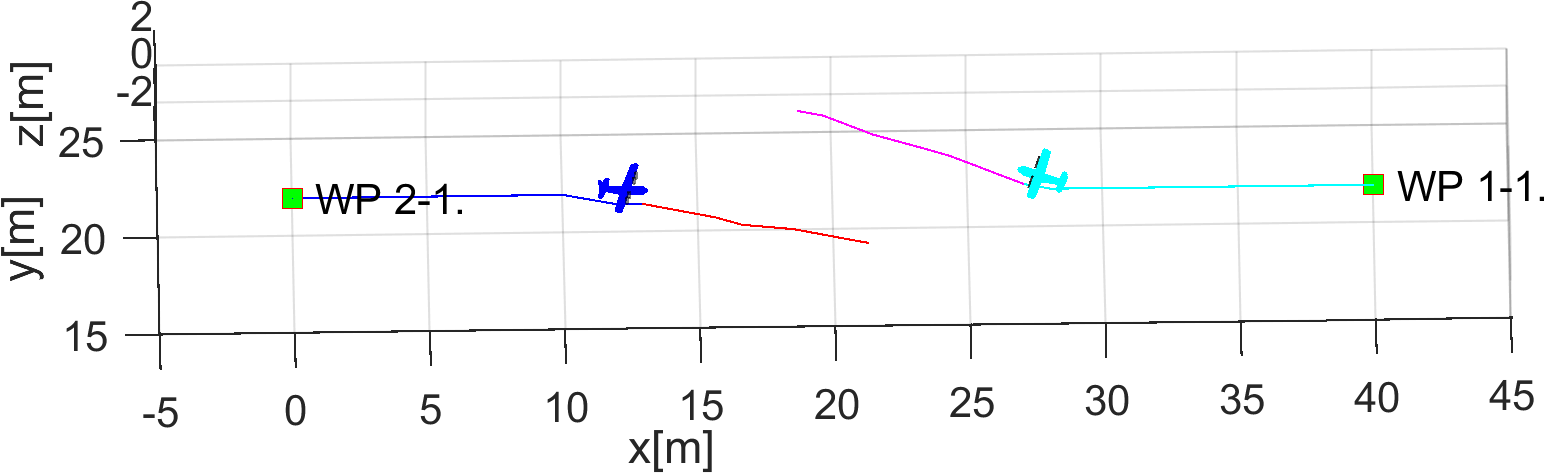
\includegraphics[width=0.9\linewidth]{\FIGDIR/NS032UtmEmergencyHeadOn00013}
        \caption{Situation detection.}
        \label{fig:emergencyHeadOnSituationDetection}
    \end{subfigure}
    \\
    \begin{subfigure}{0.75\textwidth}
        \centering
        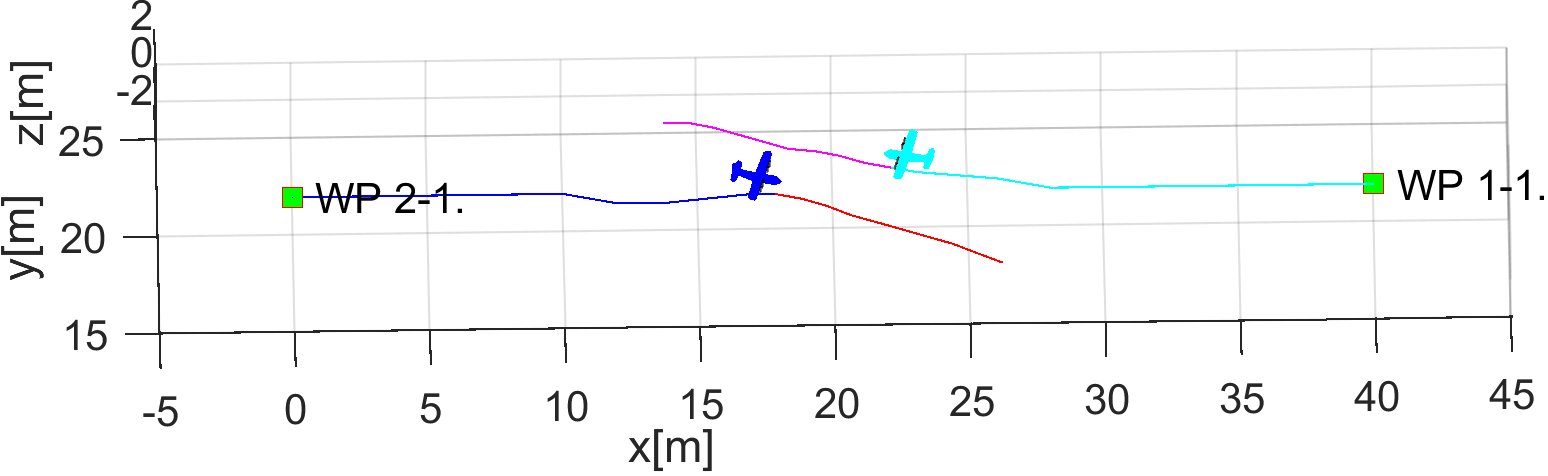
\includegraphics[width=0.9\linewidth]{\FIGDIR/NS033UtmEmergencyHeadOn00018} 
        \caption{Before near miss.}
        \label{fig:emergencyHeadOnBeforeNearMiss}
    \end{subfigure}
    \\
    \begin{subfigure}{0.75\textwidth}
        \centering
        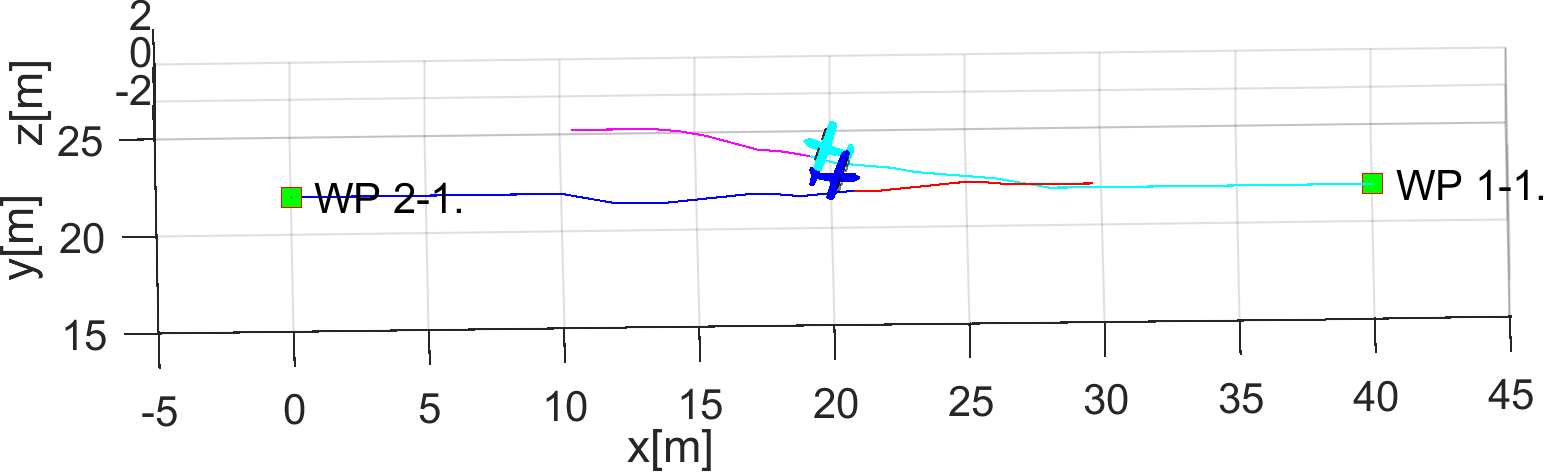
\includegraphics[width=0.9\linewidth]{\FIGDIR/NS034UtmEmergencyHeadOn00021} 
        \caption{Near-miss.}
        \label{fig:emergencyHeadOnNearMiss}
    \end{subfigure}
    \\
    \begin{subfigure}{0.75\textwidth}
        \centering
        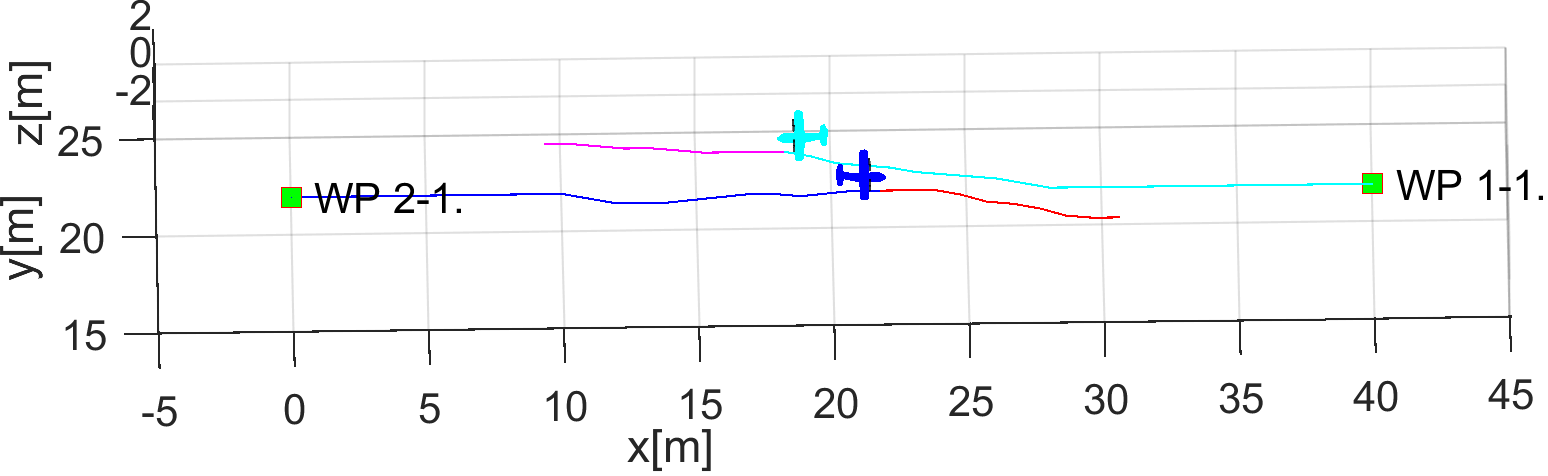
\includegraphics[width=0.9\linewidth]{\FIGDIR/NS035UtmEmergencyHeadOn00022} 
        \caption{After near miss.}
        \label{fig:emergencyHeadOnAfterNearMiss}
    \end{subfigure}
    \caption{Test scenario for \emph{Emergency head-on approach} (Intruder avoidance). }
    \label{fig:testCaseEmergencyHeadOnApproach}
\end{figure}


\paragraph{Distance to Safety Margin Evolution:} There is a need to compare the mutual distance between both UAS (y-axis [m]) and its evolution over synchronized \emph{UTM time} (x-axis [s].) The \emph{mutual distance} between bodies of \emph{UAS 1}, \emph{UAS 2} (blue line) compared to \emph{Safety Margin} (red line) is given in (fig. \ref{fig:testCaseHeadOnAvoidancePerformance}). The \emph{Safety Margin} value was constant for all time at value $1.2$ $m$ which is double of \emph{Near Miss Margin for UAS 1 UAS 2}.

The proper \emph{Avoidance Invocation} is shown when \emph{UAS} systems are getting closer to each other, and they start their \emph{separation phase} (Emergency Avoidance Mode switch). The mutual distance (blue line) does not cross \emph{safety margin} (red line).

\begin{figure}[H]
    \centering
    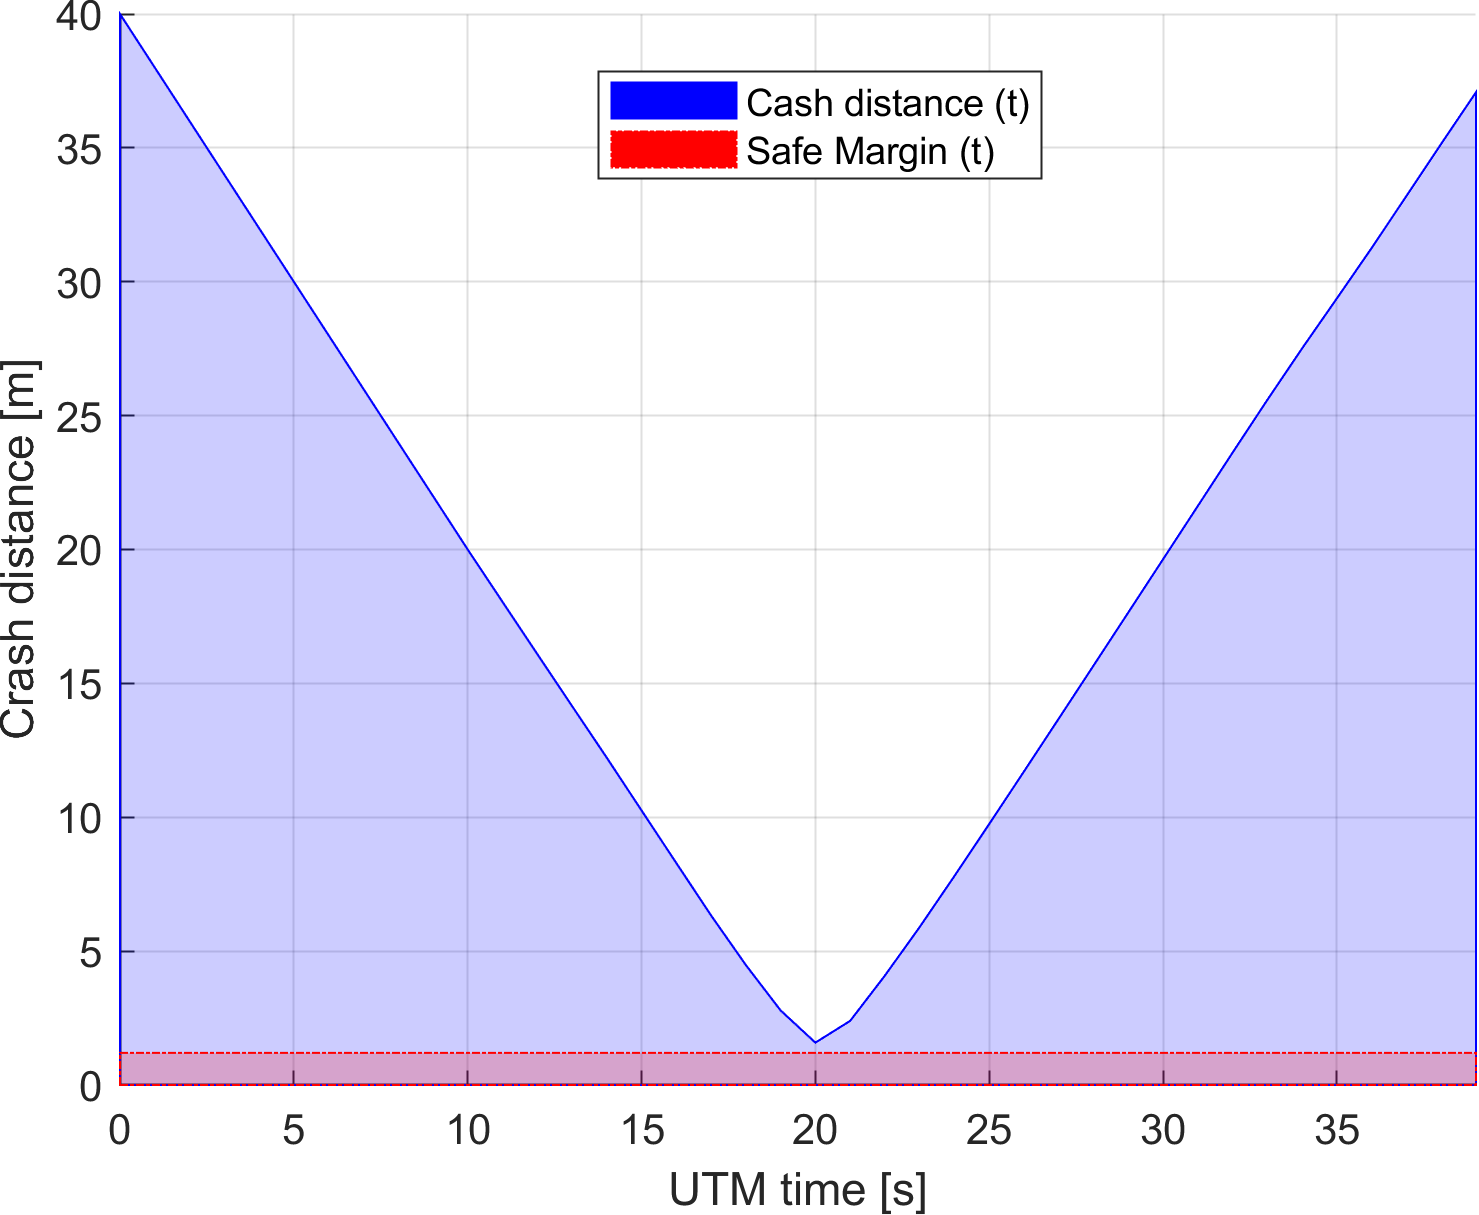
\includegraphics[width=0.55\linewidth]{\FIGDIR/NS036UtmEmergencyHeadOnPerformance} 
    \caption{Distance to safety margin evolution for \emph{emergency head-on scenario}.}
    \label{fig:testCaseHeadOnAvoidancePerformance}
\end{figure}


\paragraph{Distance to Safety Margin Peaks:} Minimal and Maximal mutual distance to safety margin is summarized in (tab. \ref{tab:testCaseEmergencyHeadOnSafetyMarginDistances}). The closest to the collision are UAS systems when the \emph{distance to safety margin} is $0.3824 m$.

The \emph{minimal distance to safety margin} $\ge$ $0$ which means that the \emph{safety acceptance criterion} is fulfilled.


\begin{table}[H]
    \centering
    \begin{tabular}{c|c||c}
    \multicolumn{2}{c||}{UAS:} & 1-2 \\\hline\hline
    \multirow{2}{*}{Distance to Safety Margin} & min & 0.3824 \\\cline{2-3}
                                            & max & 38.8000 \\
    \end{tabular}
    \caption{Distance to safety margin peaks for \emph{Emergency head-on scenario}.}
    \label{tab:testCaseEmergencyHeadOnSafetyMarginDistances}
\end{table}

\paragraph{Path Tracking Performance} All waypoints (green numbered squares) for both UAS have been reached (fig. \ref{fig:emergencyHeadOnTrajectoryTrackingPerformance}). \emph{Reference trajectories} (green dashed lines), between the initial position (green square marked S) and goal waypoint (green square marked 1) are split into three XYZ values with respective figures. The tracked value is on y-axis [m] and time on x-axis [s]. The blue lines represent real parameter evolution over time.

Following observations can be made from path tracking (fig.\ref{fig:emergencyHeadOnTrajectoryTrackingPerformance}) and preferred separations (tab. \ref{tab:aboidanceParametersForEmergencyHeadOnScenario}):

\begin{enumerate}
    \item UAS 1 (fig. \ref{fig:emergencyHeadOnUAS1PathTracking}) is using horizontal separation going to the right (y-axis) and a little bit up (z-axis).
    
    \item UAS 2 (fig. \ref{fig:emergencyHeadOnUAS2PathTracking}) is using horizontal separation going to the right (left in GCS, y-axis) and a little bit up (z-axis).
\end{enumerate}

\begin{figure}[H]
	\centering
    \begin{subfigure}{0.48\textwidth}
    	\centering
        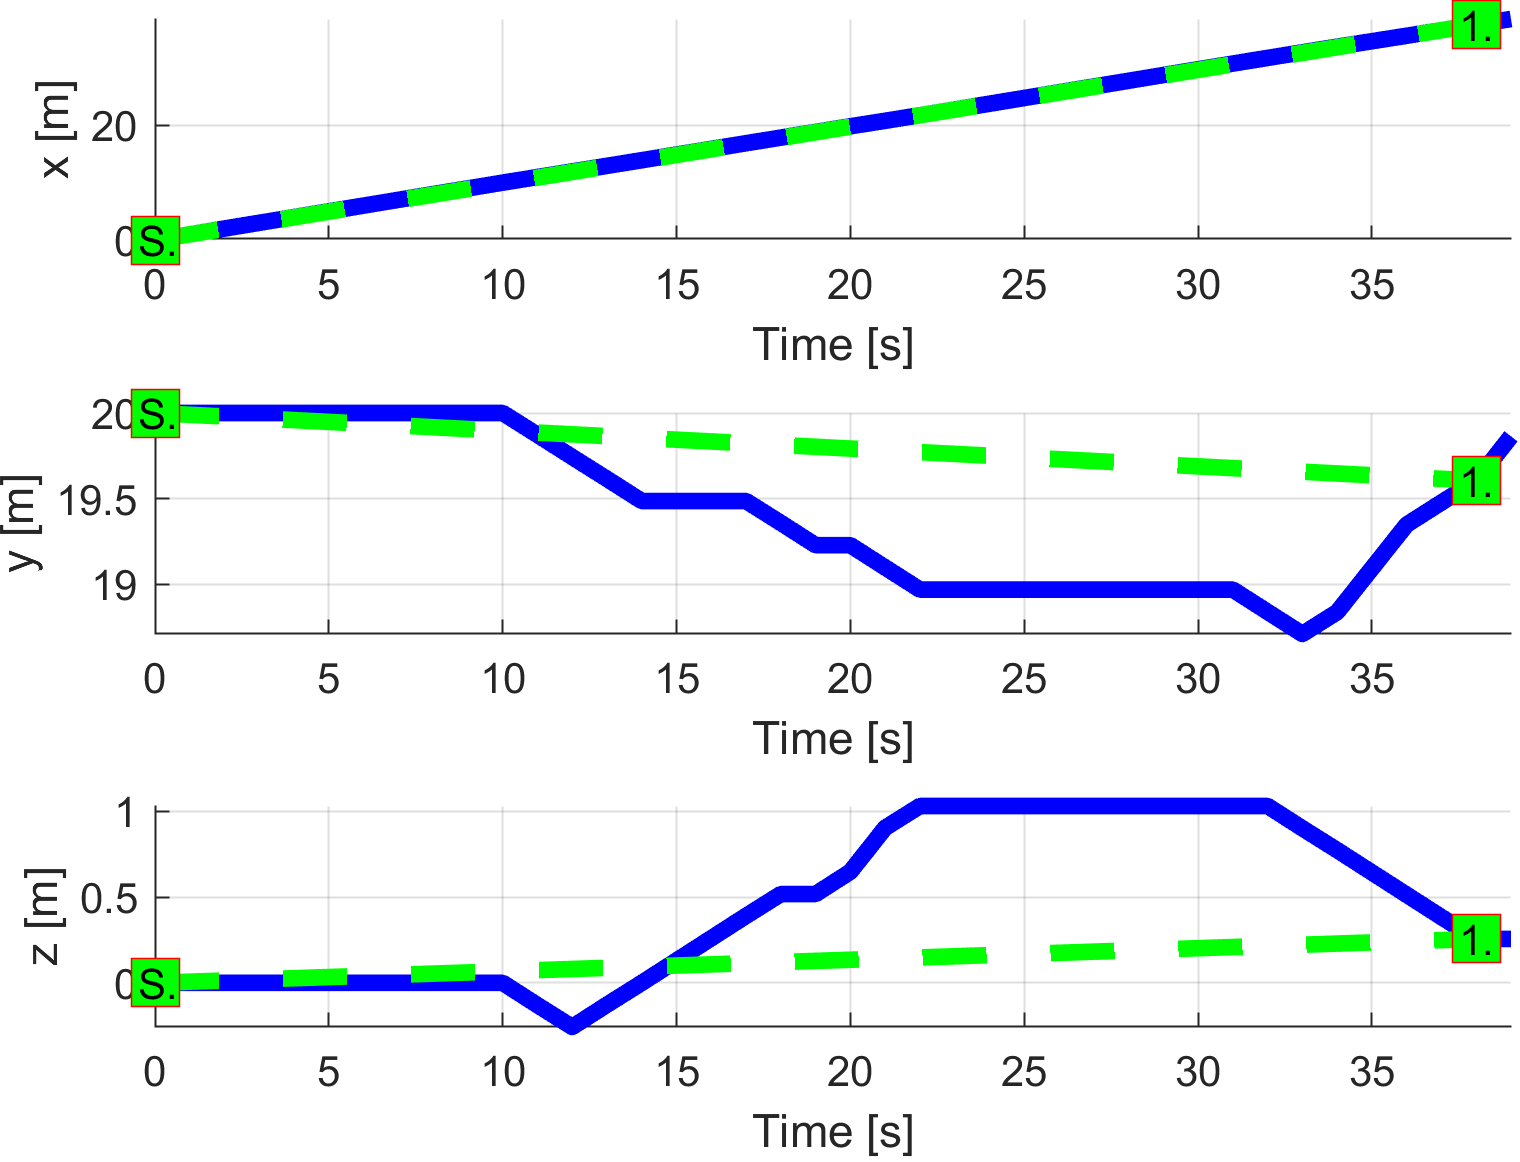
\includegraphics[width=0.9\linewidth]{\FIGDIR/NS037UtmEmergencyHeadOnUAV1PathFollowing}
        \caption{UAS 1.}
        \label{fig:emergencyHeadOnUAS1PathTracking}
    \end{subfigure}
    \begin{subfigure}{0.48\textwidth}
    	\centering
        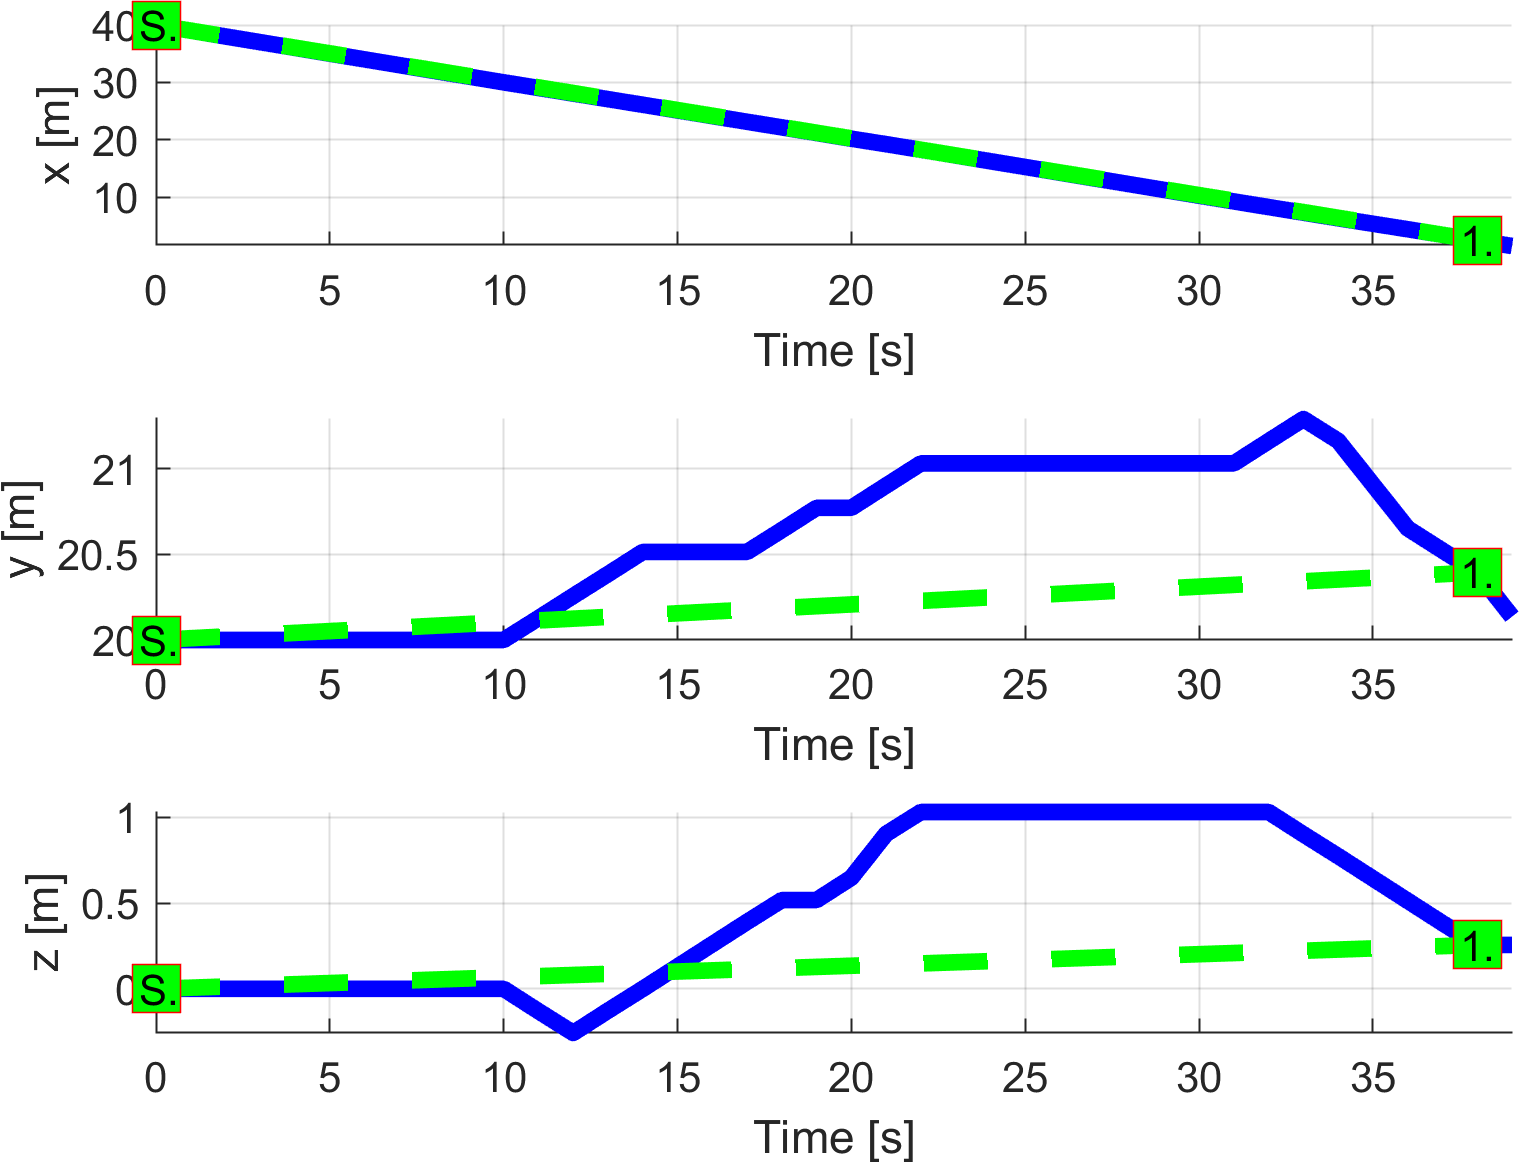
\includegraphics[width=0.9\linewidth]{\FIGDIR/NS038UtmEmergencyHeadOnUAV2PathFollowing} 
        \caption{UAS 2.}
        \label{fig:emergencyHeadOnUAS2PathTracking}
    \end{subfigure}
    \caption{\emph{Trajectory tracking} for \emph{Emergency head-on} test case. }
    \label{fig:emergencyHeadOnTrajectoryTrackingPerformance}
\end{figure}


\paragraph{Path Following Deviations:} \emph{Deviations} (tab. \ref{tab:pathTrackingParametersForEmergencyHeadOn}) are in expected ranges considering the \emph{mission plans} (tab. \ref{tab:missionSetupEmergencyHeadOnScenario}) and \emph{separation safety margins} (tab. \ref{tab:aboidanceParametersForEmergencyHeadOnScenario}).


\begin{table}[H]
    \centering
    \begin{tabular}{c||c|c}
        \multirow{2}{*}{Param.} & UAS 1     & UAS 2\\\cline{2-3}
                        & $\mathscr{WP}_1$  & $\mathscr{WP}_1$\\\hline\hline
          $\max |x|$    & 0.05              & 0.06 \\\hline
          $\max |y|$    & 1.37              & 1.48 \\\hline
          $\max |z|$    & 1.03              & 1.05 \\\hline
          $\max dist.$  & 1.39              & 1.52 \\
    \end{tabular}
    \caption{Path tracking properties for \emph{Emergency head-on} scenario.}
    \label{tab:pathTrackingParametersForEmergencyHeadOn}
\end{table}

% 06 Emergency Head On
\paragraph{Computation Load:} The \emph{computation load} for \emph{scenario} (fig.\ref{fig:emergencyConvergingComputationTime}) shows used time (y-axis) over decision frame (x-axis).

The \emph{computation time} is increased only during the \emph{avoidance phase}. The \emph{load} is symmetric for both UAS systems.

\begin{figure}[H]
    \centering
    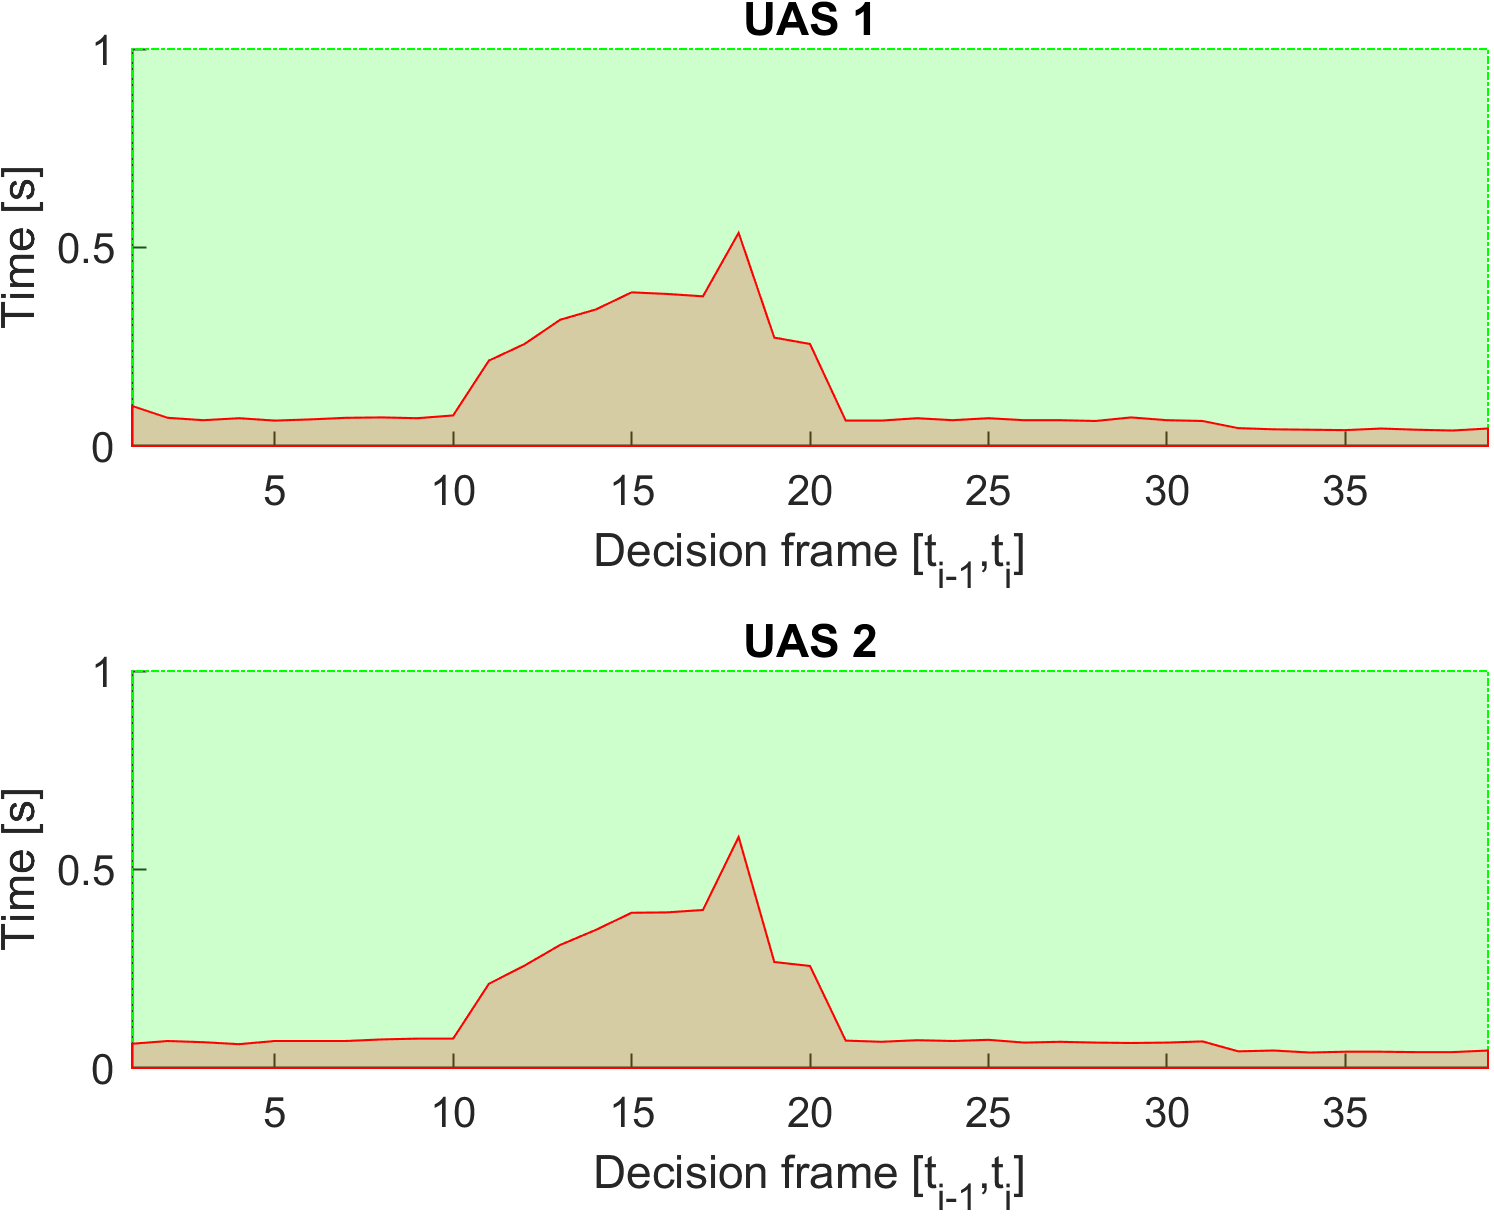
\includegraphics[width=0.50\linewidth]{\FIGDIR/NS097EmergencyHeadOnComputationTime} 
    \caption{Computation time for \emph{Emergency head-on} scenario.}
    \label{fig:emergencyHeadOnComputationTime}
\end{figure}